\section{Phase Structure}
\label{sec:phase}

The dynamics of the causal log network do not produce uniform behavior.
Depending on the magnitude of the effective coupling, the network
operates in qualitatively different regimes.
Physical laws are properties of a specific phase,
not universal principles valid across all parameter regimes.

\subsection{The Control Parameter}

The key parameter is:

\begin{equation}
  \alpha_i = \lambda\,h_i,
  \qquad
  h_i = \sum_j H_{ij},
  \label{eq:alpha}
\end{equation}

where $\lambda$ is the selection sensitivity and $h_i$ is the total
incoming causal history at node $i$.
At $\alpha_i = 1$, a bifurcation occurs: below this value no log density
can be self-sustained; above it, $\rho_i$ rises and structure forms.
The phase structure is shown in Fig.~\ref{fig:phase_structure}.

\begin{figure}[t]
\centering
\setcounter{figure}{1}
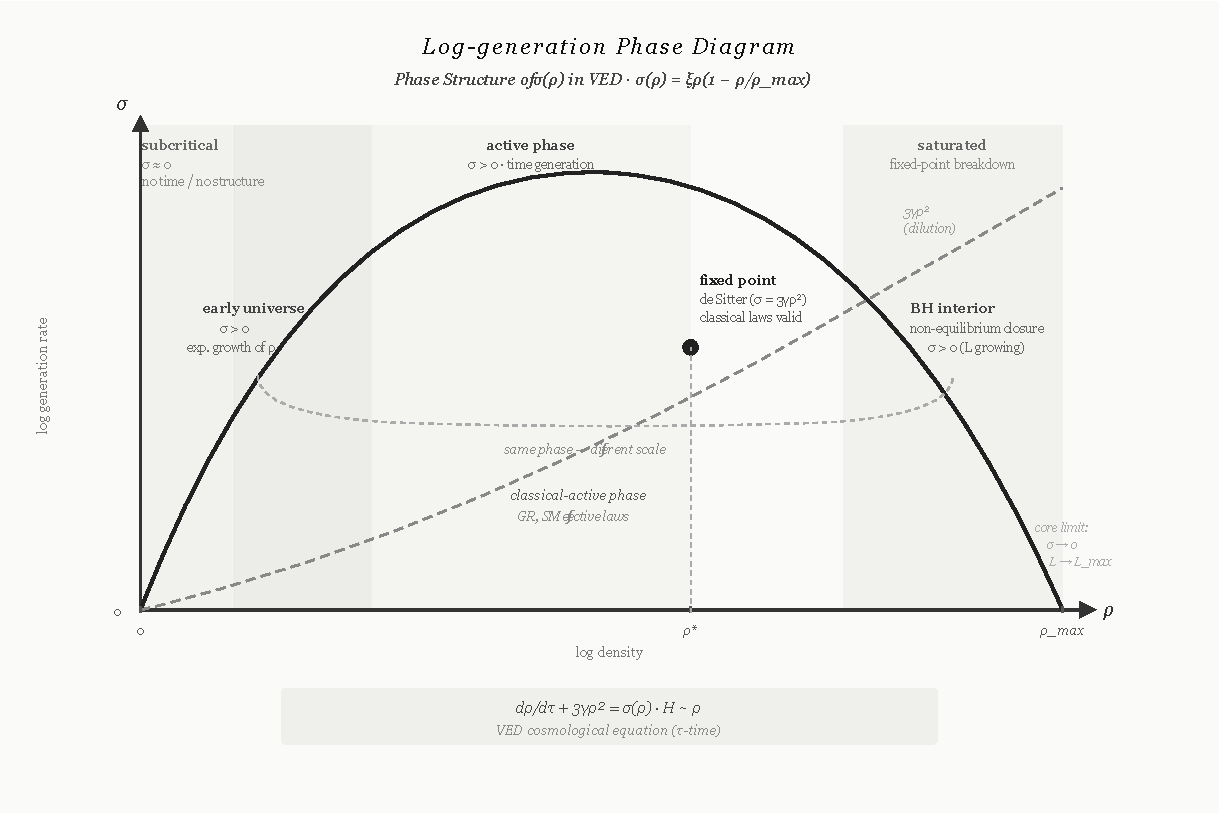
\includegraphics[width=0.85\linewidth]{figures/fig2_phase_diagram.pdf}
\caption{
Phase structure as a function of density $\rho$.
The system transitions across subcritical, critical, classical-active,
and saturated regimes. Physical laws emerge as properties of stable phases.
}
\label{fig:phase_structure}
\end{figure}

\subsection{Four Phases}

\begin{table}[h]
\centering
\begin{tabular}{llp{7cm}}
\toprule
Phase & Condition & Character \\
\midrule
Subcritical   & $\alpha < 1$     & $\rho \approx 0$; no time, no structure \\
Critical      & $\alpha = 1$     & Maximum susceptibility; bifurcation point \\
Classical-active & $\alpha \sim 1$ & Stable closures; effective laws emerge \\
Saturated     & $\alpha \gg 1$   & $C_{ij} \to 1$; differences vanish \\
\bottomrule
\end{tabular}
\caption{Phase structure of the causal log network.}
\label{tab:phases}
\end{table}

\subsection{Emergence of Physical Laws}

Within the classical-active phase, the following structures become stable:

\begin{itemize}
  \item \textbf{Conservation laws}: $\sigma \approx 0$, so
    $\partial_t\rho + \nabla\cdot\mathbf{J} \approx 0$.
  \item \textbf{Gauge symmetries}: closure configurations stabilize with
    well-defined internal degrees of freedom (Vol.~2).
  \item \textbf{Effective geometry}: coarse-grained distance $d_{ij}$ becomes
    approximately smooth, admitting a metric tensor $g_{\mu\nu}$ (Vol.~3).
\end{itemize}

\begin{keybox}
\textit{Conservation, symmetry, and geometry are properties of the
classical-active phase --- not axioms.
They emerge within it and break down outside it.}
\end{keybox}

\subsection{Extreme Regimes as Phase Transitions}

The framework naturally accommodates extreme regimes:

\begin{itemize}
  \item \textbf{Big Bang}: transition from subcritical to active phase.
    Structure bootstraps from a region where $\alpha$ crosses the critical
    threshold --- not from a geometric singularity.
  \item \textbf{Black hole interiors}: transition from classical-active to
    non-equilibrium phase. The interior is not a singularity;
    it is a regime where fixed-point conditions break down
    and $\sigma > 0$ reignites (Vol.~3).
\end{itemize}
